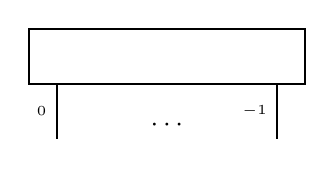
\begin{tikzpicture}[scale=0.35, thick] % , baseline = -3.5pt

    %	\draw[->] (0,1)--(0,3) node[midway,left] {$\atomlegindexof{\exformula}$};
	
    	\draw (-5,1) rectangle (5,-1);
    	\node[anchor=center] at (0,0) {\small ${\groundingof{\exformula}}$} ;
    	\draw[] (-4,-1)--(-4,-3) node[midway,left] {\tiny $\exindividualof{0}$};
    	\draw[] (4,-1)--(4,-3) node[midway,left] {\tiny $\exindividualof{\variableorder-1}$};
    	\node at (0,-3.1) [above] {$\cdots$};
    
\end{tikzpicture}